\documentclass[a4paper, 11pt]{article}
\usepackage[english]{babel}
\usepackage[T1]{fontenc}
\usepackage[utf8]{inputenc}

% Import images from media folder.
\usepackage{graphicx}
\graphicspath{ {./media/} }

% Header & Footer
% \usepackage{fancyhdr}
% \pagestyle{fancy}
% \lhead{Konrad M. L. Claesson}

\usepackage{soul, color} % Strikethrough, highlight
\usepackage{enumitem} % Enumerate using letters, a) b) c), ...

% No default paragraph indentation.
\setlength{\parindent}{0px}
\renewcommand{\baselinestretch}{1.325}

% Change Paragraph Spacing
\usepackage{setspace}

% Double quotes, \say{}.
\usepackage{dirtytalk}

% Block quotes
\usepackage{etoolbox}
\AtBeginEnvironment{quote}{\singlespacing\small}

% Links
\usepackage{hyperref}
\definecolor{urlblue}{RGB}{000, 106, 219}
\hypersetup{
   colorlinks=true,  % false: boxed links; true: colored links
   linkcolor=black,  % color of internal links
   urlcolor=urlblue
}

% 1st, 2nd, ...
\usepackage{nth}

% Tables
\usepackage{longtable}
\usepackage{float}

% General Math
\usepackage{amsmath}

% Proofs
\usepackage{logicproof}

% Code
\usepackage{fancyvrb}
\usepackage{listings}

\lstset
{
  basicstyle=\small\ttfamily,
  breaklines=true,
  columns=fullflexible
}

% Cover Page
\title{CTL Model Checking}
\author
{
   Konrad M. L. Claesson \\
   konradcl@kth.se \\
   Lab 3 $-$ DD1351
}
\date{\today}

\begin{document}
   \maketitle
   \thispagestyle{empty}   % remove page number
   
   % Restart numbering
   \clearpage
   \pagenumbering{arabic}
   \newpage

   \tableofcontents
   \newpage

   \section{Introduction}

   There are numerous proof-based and model-based
   verification techniques that can be used to verify the
   correctness of computer systems. Computer Tree Logic (CTL)
   is a branching-time logic that represents a system by a set
   of states and a set of possible transitions between the 
   states. It can be used to model a system that transitions
   between states over time. Moreover, a model checker can
   be implemented to verify that the system satisfies a set
   of desired properties.
   \bigbreak

   This report starts out by introducing a Prolog-based
   model checker for the following subset of CTL rules (see
   Figure \ref{ctl-proof-system} for rule definitions):
   $$\phi ::= p 
      \mid \neg p 
      \mid \phi \wedge \phi
      \mid \phi \vee \phi
      \mid \text{AX} \, \phi
      \mid \text{AG} \, \phi
      \mid \text{AF} \, \phi
      \mid \text{EX} \, \phi
      \mid \text{EG} \, \phi
      \mid \text{EF} \, \phi
   $$
   Then, the model checker is used to verify two properties 
   of a CTL model of an elevator. 

   \section{Method}
   
   The model checker takes its input from a file that includes
   a list of state-\say{formula set} pairs that corresponds 
   to a labeling function; another list of 
   state-\say{state set} pairs that specifies all possible 
   transitions from one state to another; a starting state 
   for the model check; and a CTL formula to verify. Then, 
   the passed in model is verified according to the rules in 
   Figure \ref{ctl-proof-system}. The implementation of each 
   rule can be found in the program code in the appendix. 
   Furthermore, tables 
   \ref{helper-predicates},
   \ref{propositional-ctl-rule-table},
   \ref{a-rule-table} and
   \ref{e-rule-table}
   lists all Prolog predicates 
   along with the conditions under which they return true.

   \begin{figure}[H]
      \centering
      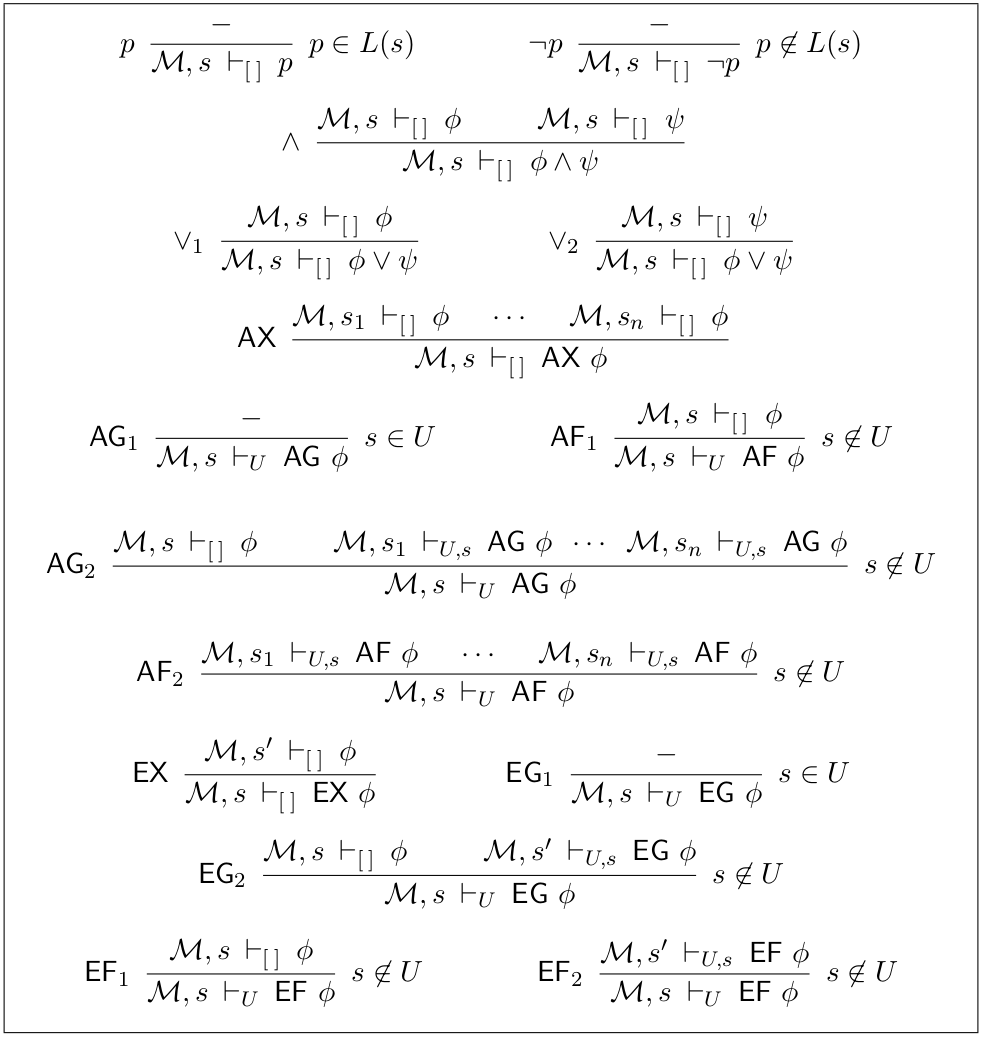
\includegraphics[scale=0.30]{ctl-proof-system}
      \caption{CTL Proof System}
      \label{ctl-proof-system}
   \end{figure}
   \bigbreak


   \subsection{The Check Predicate}
   The \texttt{check/5} predicate takes in a
   transition function (called \texttt{Transitions}), 
   a \texttt{Labeling} function, a current 
   \texttt{State}, a list of previously visited states 
   (called \texttt{PastStates}), and a formula to verify
   (called \texttt{Formula} or \texttt{X}). 
   The term \say{function} is used loosely here; in
   the program, \texttt{Transitions} and \texttt{Labeling}
   are implemented as lists of pairs. \texttt{check/5}
   proceeds to verify the passed in formula by ensuring that
   it follows the CTL rules defined in figure
   \ref{ctl-proof-system}.
   \bigbreak

   The following table describes the \texttt{verify/1}
   predicate along with two helper predicates that are
   frequently used in the model checker.

\begin{table}[H]
\centering
\begin{tabular}{|l|l|l|}
   \hline
      \textbf{Predicate} 
      & \textbf{Parameters}                                  
      & \textbf{Description} \\
   \hline
      \texttt{verify}             
      & \texttt{InputFileName}  
      & \begin{tabular}[c]{@{}l@{}}
         \texttt{verify} returns true when \\ 
         the formula in the input \\ 
         file is verified by \texttt{check/5}.
      \end{tabular} \\  
   \hline
      \texttt{get\_state\_formulas}       
      & \begin{tabular}[c]{@{}l@{}}
         \texttt{Labeling} \\ 
         \texttt{State} \\ 
         \texttt{Formulas}
      \end{tabular}          
      & \begin{tabular}[c]{@{}l@{}}
         True whenever a list of the \\ 
         form \texttt{[State, \_]} exists in \\ 
         \texttt{Labling}. This predicate is \\ 
         used to get the \texttt{Formulas} \\ 
         that are true in \texttt{State}. 
      \end{tabular} \\  
   \hline
      \texttt{get\_adjacent\_states}        
      & \begin{tabular}[c]{@{}l@{}}
         \texttt{Transitions} \\ 
         \texttt{State} \\
         \texttt{AdjacentStates}
      \end{tabular}                    
      & \begin{tabular}[c]{@{}l@{}}
         Returns true if a list of the \\
         form \texttt{[State, \_]} exists in \\
         \texttt{AdjacentStates}. This \\ 
         predicate is used to get the \\ 
         states to which it is possible \\ 
         to transition from \texttt{State}.
      \end{tabular} \\  
   \hline
\end{tabular}
\caption{Entry Point and Helper Predicates}
\label{helper-predicates}
\end{table}

   The CTL rules of figure \ref{ctl-proof-system} can be 
   subdivided into \textit{propositional} rules, 
   \textit{A}-rules and \textit{E}-rules. Each of these 
   categories are explored in the subsections ahead.

   \subsubsection{Propositional Rules}
   \label{propositional-rules}
   The propositional rules of CTL are 
   $\phi ::= p \mid \neg p \mid \phi \wedge \phi \mid \phi
   \vee \phi$
   and are implemented by checking whether the formula to be
   verified is a member of the formulas that are \texttt{true}
   in the current state. For example,

\begin{verbatim}
   check(_, Labling, State, [], Formula) :-
      get_state_formulas(Labling, State, Formulas),
      member(Formula, Formulas).
\end{verbatim}

   verifies that \texttt{Formula} is \texttt{true}.
   \bigbreak

   The below table describes under what conditions the check
   predicates for each of the propositional rules are true.
   \bigbreak

   \begin{longtable}[H]{|l|l|l|}
      \hline
         \textbf{CTL Rule}
         & \textbf{Truth Conditions} \\
      \hline
         \texttt{p} 
         & \begin{tabular}[c]{@{}l@{}}
            The check predicate evaluates to true if 
            \texttt{p} \\
            is a member of the formulas on the given state.
         \end{tabular} \\
      \hline
         \texttt{neg(p)} 
         & \begin{tabular}[c]{@{}l@{}}
            The check predicate evaluates to true if 
            \texttt{p} \\
            is \textit{not} a member of the formulas on the 
            given state.
         \end{tabular} \\
      \hline
         \texttt{and(X,Y)} 
         & \begin{tabular}[c]{@{}l@{}}
            The check predicate evaluates to true if both \\ 
            \texttt{X} and \texttt{Y}
            are members of the given state.
         \end{tabular} \\
      \hline
         \texttt{or(X,\_)} 
         & \begin{tabular}[c]{@{}l@{}}
            The check predicate evaluates to true if 
            \texttt{X} is a \\ 
            member of the given state.
         \end{tabular} \\
      \hline
         \texttt{or(\_,Y)} 
         & \begin{tabular}[c]{@{}l@{}}
            The check predicate evaluates to true if 
            \texttt{Y} is a \\ 
            member of the given state.
         \end{tabular} \\
      \hline
         \texttt{or(\_,Y)} 
         & \begin{tabular}[c]{@{}l@{}}
            The check predicate evaluates to true if 
            \texttt{Y} is a \\ 
            member of the given state.
         \end{tabular} \\
      \hline
   \caption{Truth Conditions for Propositional CTL Rules}
   \label{propositional-ctl-rule-table}
   \end{longtable}

   \subsubsection{\textit{A}-Rules}
   \label{a-rules}

   The CTL rules referred to as \textit{A}-rules in this
   report are 
   $$
      \phi ::= \text{AX} \, \phi 
      \mid \text{AG} \, \phi 
      \mid \text{AF} \, \phi
   $$
   and all share the commonality that the condition that they
   impose must be \texttt{true} \textit{along all paths}.
   Another commonality is that all \textit{A}-rules leverage
   the \texttt{check\_all/5} predicate, which has the
   implementation

\begin{verbatim}
check_all(_, _, [], _, _).
check_all(Transitions, Labling, [State|States], PastStates, X) :-
   check(Transitions, Labling, State, PastStates, X),
   check_all(Transitions, Labling, States, PastStates, X).
\end{verbatim}

   and checks that all states, i.e. \texttt{[State|States]}
   from the code, satisfy the formula \texttt{X}. The 
   following table states under what conditions the 
   \texttt{check/5} predicates for the \textit{A}-rules 
   return \texttt{true}.
   \bigbreak

   \begin{longtable}[ht]{|l|l|l|}
      \hline
         \textbf{CTL Rule}
         & \textbf{Truth Conditions} \\
      \hline
         \texttt{ax(X)} 
         & \begin{tabular}[c]{@{}l@{}}
            The check predicate evaluates to \texttt{true} if 
            \texttt{X} is \texttt{true} \\ 
            in any state to which there exists
            an immediate \\ 
            transition from the current state.
         \end{tabular} \\
      \hline
         \texttt{ag(X)} 
         & \begin{tabular}[c]{@{}l@{}}
            The check predicate evaluates to \texttt{true} if 
            \texttt{X} is \texttt{true} \\ 
            in all states.
         \end{tabular} \\
      \hline
         \texttt{af(X)} 
         & \begin{tabular}[c]{@{}l@{}}
            The check predicate evaluates to \texttt{true} if 
            \texttt{X} is \\ 
            eventually true in some state along any path.
         \end{tabular} \\
      \hline
      \caption{Truth Conditions for CTL \textit{A}-Rules}
      \label{a-rule-table}
   \end{longtable}

   \subsubsection{\textit{E}-Rules}
   \label{e-rules}
   
   The CTL rules referred to as \textit{E}-rules in this
   report are 
   $$
      \phi ::= \text{EX} \, \phi 
      \mid \text{EG} \, \phi 
      \mid \text{EF} \, \phi
   $$
   and all share the commonality that the condition that they
   impose must be \texttt{true} \textit{along some path}.
   Another commonality is that all \textit{E}-rules leverage
   the \texttt{find\_state/5} predicate, which has the
   implementation

\begin{verbatim}
find_state(Transitions, Labling, [State|States], PastStates, X) :-
   check(Transitions, Labling, State, PastStates, X);
   find_state(Transitions, Labling, States, PastStates, X).
\end{verbatim}

   and checks if there exists a state in 
   \texttt{[State|States]} where the formula \texttt{X} is
   satisfied. The subsequent table states under what
   conditions the \texttt{check/5} predicates for the
   \textit{E}-rules return \texttt{true}.
   \bigbreak

   \begin{longtable}[ht]{|l|l|l|}
      \hline
         \textbf{CTL Rule}
         & \textbf{Truth Conditions} \\
      \hline
         \texttt{ex(X)} 
         & \begin{tabular}[c]{@{}l@{}}
            The check predicate evaluates to \texttt{true} if 
            \texttt{X} is \texttt{true} \\
            in some state to which there exists
            an immediate \\ 
            transition from the current state.
         \end{tabular} \\
      \hline
         \texttt{eg(X)} 
         & \begin{tabular}[c]{@{}l@{}}
            The check predicate evaluates to \texttt{true} if 
            there \\ 
            exists a path along which \texttt{X} is 
            \texttt{true} in all states.
         \end{tabular} \\
      \hline
         \texttt{ef(X)} 
         & \begin{tabular}[c]{@{}l@{}}
            The check predicate evaluates to \texttt{true} if 
            there \\
            exists a path where \texttt{X} is
            \texttt{true} eventually.
         \end{tabular} \\
      \hline
      \caption{Truth Conditions for CTL \textit{E}-Rules}
      \label{e-rule-table}
   \end{longtable}

   \subsection{Elevator Model}
   An elevator traveling between two floors was modeled and
   tested using the described model checker. The following
   atomic propositions are used in the model:

   \begin{itemize}
      \item \texttt{floor1}: The elevator is on the first
         floor.
      \item \texttt{floor2}: The elevator is on the second
         floor.
      \item \texttt{open}: The elevator doors are open.
      \item \texttt{closed}: The elevator doors are closed.
      \item \texttt{opening}: The elevator doors are opening.
      \item \texttt{closing}: The elevator doors are closing.
      \item \texttt{still}: The elevator is not moving.
      \item \texttt{btn1}: The elevator button to go to the
         first floor is toggled on.
      \item \texttt{btn2}: The elevator button to go to the
         second floor is toggled on.
   \end{itemize}
   
   The elevator was modeled with the states $S := \{s_0, s_1,
   \dots, s_{13}\}$, labeling function
   \begin{equation*}
   \begin{split}
   L := \{ 
   (s0, \{\texttt{floor1}, \texttt{open}, \texttt{still}\}),
      \\
   (s1, \{\texttt{floor1}, \texttt{open}, \texttt{still},
      \texttt{btn2}\}), \\
   (s2, \{\texttt{floor1}, \texttt{closing}, \texttt{still},
      \texttt{btn2} \}), \\
   (s3, \{\texttt{floor1}, \texttt{closed}, \texttt{still},
      \texttt{btn2}\}), \\
   (s4, \{\texttt{closed}, \texttt{still}, \texttt{still}\}),
      \\
   (s5, \{\texttt{floor2}, \texttt{closed}, \texttt{still}\}),
      \\
   (s6, \{\texttt{floor2}, \texttt{opening},
      \texttt{still}\}), \\
   (s7, \{\texttt{floor2}, \texttt{open}, \texttt{still}\}), 
      \\
   (s8, \{\texttt{floor2}, \texttt{open}, \texttt{still},
      \texttt{btn1}\}), \\
   (s9, \{\texttt{floor2}, \texttt{closing}, \texttt{still},
      \texttt{btn2}\}), \\
   (s10, \{\texttt{floor2}, \texttt{closed}, \texttt{still},
      \texttt{still}, \texttt{btn2}\}\}), \\
   (s11, \{\texttt{closed}, \texttt{down}, \texttt{btn1}\}),
      \\
   (s12, \{\texttt{floor1}, \texttt{closed},
      \texttt{still}\}), \\
   (s13, \{\texttt{floor1}, \texttt{openning},
      \texttt{still}\})
   \},
   \end{split}
   \end{equation*}

   and transition function

   \begin{equation*}
   \begin{split}
   \rightarrow := \{ 
   (s_0, \{s_0, s_1\}), (s_1, \{s_0, s_1, s_2\}), 
      (s_2, \{s_3, s_{13}\}), \\
   (s_3, \{s_4\}), (s_4, \{s_5\}), (s_5, \{s_6\}), \\
   (s_6, \{s_7\}), (s_7, \{s_7, s_8\}), 
      (s_8, \{s_7, s_8, s_9\}), \\
   (s_9, \{s_{10}, s_6\}), (s_{10}, \{s_{11}\}), 
      (s_{11}, \{s_{12}\}), \\
   (s_{12}, \{s_{13}\}), (s_{13}, \{s_0\})
   \}.
   \end{split}
   \end{equation*}

   As previously, the term \say{function} is used loosely
   here; $L$ and $\rightarrow$ are actually sets of pairs.
   \bigbreak

   The model was tested for two formulas: 
   \begin{itemize}
      \item \texttt{ef(and(and(floor2, open), still))}
      \item \texttt{ef(and(neg(still), or(open, or(opening,
         closing))))}
   \end{itemize}

   The first formula states that \say{from the current state
   (which has to be specified), there exists a path where,
   eventually, $\texttt{floor2} \wedge \texttt{open} \wedge
   \texttt{still}$ is \texttt{true}.} In other words, it is
   possible to use the elevator to get to the second floor.
   The formula was be tested starting from state 
   $s_0$ (an idle elevator on the first floor) and was 
   expected to evaluate to \texttt{true}.
   \bigbreak

   The second formula states that \say{from the current state,
   there exists a path where, eventually, 
   $\neg \texttt{still} \wedge (\texttt{open} \vee
   \texttt{opening} \vee \texttt{closing})$ is \texttt{true}}.
   Phrased differently, the formula states that there exists
   a state where the elevator is moving while its doors are
   not closed. The formula was tested from state $s_0$ and
	was expected to return \texttt{false}.

   \section{Results}
   
   The model checker was tested with 32 unit tests that test
	each of the CTL rules in isolation on models with a minimal
	number of propositions, states and transitions. All unit
   tests passed. The model checker was also tested with 905
   more complex integration tests. All integration tests
   passed too.
   \bigbreak

   The formulas that were tested for the elevator model ended
   up evaluating to the expected boolean values.
   \texttt{ef(and(and(floor2, open), still))} returned
   \texttt{true} and 
   \texttt{ef(and(neg(still), or(open, or(opening, closing))))
   } returned \texttt{false}.
   \bigbreak

   The model checker along with the elevator model and tests 
   can be found by following this link:
   \url{github.com/konradcl/ctl-model-checker}. The
   model checker and tests for the above elevator model
   formulas have also been appended to this report.

   \newpage
   \section{Appendix}

   \subsection{Input File for Testing 
      \texttt{ef(and(and(floor2, open), still))}}

\begin{lstlisting}
% Transition Function
[
   [s0, [s0, s1]],
   [s1, [s0, s1, s2]],
   [s2, [s3, s13]],
   [s3, [s4]],
   [s4, [s5]],
   [s5, [s6]],
   [s6, [s7]],
   [s7, [s7, s8]],
   [s8, [s7, s8, s9]],
   [s9, [s10, s6]],
   [s10, [s11]],
   [s11, [s12]],
   [s12, [s13]],
   [s13, [s0]]
].

% Labling Function
[
   [s0, [floor1, open, still]],
   [s1, [floor1, open, still, btn2]],
   [s2, [floor1, closing, still, btn2]],
   [s3, [floor1, closed, still, btn2]],
   [s4, [closed, up, btn2]],
   [s5, [floor2, closed, still]],
   [s6, [floor2, opening, still]],
   [s7, [floor2, open, still]],
   [s8, [floor2, open, still, btn1]],
   [s9, [floor2, closing, still, btn1]],
   [s10, [floor2, closed, still, btn2]],
   [s11, [closed, down, btn1]],
   [s12, [floor1, closed, still]],
   [s13, [floor1, opening, still]]
].

% Initial State
s0.

% Formula to Verify
ef(and(and(floor2, open), still)).
\end{lstlisting}

   \subsection{Input File for Testing
      \texttt{ef(and(neg(still), or(open, or(opening,
         closing))))}}

\begin{lstlisting}
% Transition Function
[
   [s0, [s0, s1]],
   [s1, [s0, s1, s2]],
   [s2, [s3, s13]],
   [s3, [s4]],
   [s4, [s5]],
   [s5, [s6]],
   [s6, [s7]],
   [s7, [s7, s8]],
   [s8, [s7, s8, s9]],
   [s9, [s10, s6]],
   [s10, [s11]],
   [s11, [s12]],
   [s12, [s13]],
   [s13, [s0]]
].

% Labeling Function
[
   [s0, [floor1, open, still]],
   [s1, [floor1, open, still, btn2]],
   [s2, [floor1, closing, still, btn2]],
   [s3, [floor1, closed, still, btn2]],
   [s4, [closed, up, btn2]],
   [s5, [floor2, closed, still]],
   [s6, [floor2, opening, still]],
   [s7, [floor2, open, still]],
   [s8, [floor2, open, still, btn1]],
   [s9, [floor2, closing, still, btn1]],
   [s10, [floor2, closed, still, btn2]],
   [s11, [closed, down, btn1]],
   [s12, [floor1, closed, still]],
   [s13, [floor1, opening, still]]
].

% Initial State
s0.

% Formula to Verify
ef(and( neg(still), or(open, or(opening, closing)) )).
\end{lstlisting}


   \subsection{Model Checker Implementation}

\begin{lstlisting}
:- (discontiguous check/5).

verify(Input) :- 
   see(Input), read(Transitions), read(Labeling),
   read(State), read(Formula), seen,
   check(Transitions, Labeling, State, [], Formula).

% Recurses through Labeling to find the Formulas of State.
get_state_formulas(Labeling, State, Formulas) :-
   member([State, Formulas], Labeling).

% Recurses through Transitions to find the adjacent states to State. 
% AdjacentStates may include State itself.
get_adjacent_states(Transitions, State, AdjacentStates) :-
   member([State, AdjacentStates], Transitions).

% FORMULA
check(_, Labeling, State, [], Formula) :-
   get_state_formulas(Labeling, State, Formulas),
   member(Formula, Formulas).
	
% NEGATION
check(_, Labeling, State, [], neg(Formula)) :-
   get_state_formulas(Labeling, State, Formulas),
   \+ member(Formula, Formulas).
	
% AND
check(Transitions, Labeling, State, [], and(X, Y)) :-
   check(Transitions, Labeling, State, [], X),
   check(Transitions, Labeling, State, [], Y).

% OR 1
check(Transitions, Labeling, State, [], or(X, _)) :-
   check(Transitions, Labeling, State, [], X).

% OR 2
check(Transitions, Labeling, State, [], or(_, Y)) :-
   check(Transitions, Labeling, State, [], Y).

% Checks that all states, i.e. [State|States], satisfy Formula.
check_all(_, _, [], _, _).
check_all(Transitions, Labeling, [State|States], PastStates, X) :-
   check(Transitions, Labeling, State, PastStates, X),
   check_all(Transitions, Labeling, States, PastStates, X).

% AX
check(Transitions, Labeling, State, [], ax(X)) :-
   get_adjacent_states(Transitions, State, AdjacentStates),
   check_all(Transitions, Labeling, AdjacentStates, [], X).

% AG1 and AG2
check(_, _, State, PastStates, ag(_)) :-
   member(State, PastStates).

check(Transitions, Labeling, State, PastStates, ag(X)) :-
   \+ member(State, PastStates),
   get_adjacent_states(Transitions, State, AdjacentStates),
   check(Transitions, Labeling, State, [], X),
   check_all(Transitions, Labeling, AdjacentStates,
      [State|PastStates], ag(X)).

% AF1 and AF2
check(Transitions, Labeling, State, PastStates, af(X)) :-
   \+ member(State, PastStates),
   check(Transitions, Labeling, State, [], X).

check(Transitions, Labeling, State, PastStates, af(X)) :-
   \+ member(State, PastStates),
   get_adjacent_states(Transitions, State, AdjacentStates),
   check_all(Transitions, Labeling, AdjacentStates,
      [State|PastStates], af(X)).

% Checks if there exists a state in [State|States] where Formula 
% is satsified.
find_state(Transitions, Labeling, [State|States], PastStates, X) :-
   check(Transitions, Labeling, State, PastStates, X);
   find_state(Transitions, Labeling, States, PastStates, X).

% EX
check(Transitions, Labeling, State, [], ex(X)) :-
   get_adjacent_states(Transitions, State, AdjacentStates),
   find_state(Transitions, Labeling, AdjacentStates, [], X).

% EG1 and EG2
check(_, _, State, PastStates, eg(_)) :-
   member(State, PastStates).

check(Transitions, Labeling, State, PastStates, eg(X)) :-
   \+ member(State, PastStates),
   check(Transitions, Labeling, State, [], X),
   get_adjacent_states(Transitions, State, AdjacentStates),
   find_state(Transitions, Labeling, AdjacentStates, 
      [State|PastStates], eg(X)).
	
% EF1 and EF2
check(Transitions, Labeling, State, PastStates, ef(X)) :-
   \+ member(State, PastStates),
   check(Transitions, Labeling, State, [], X).

check(Transitions, Labeling, State, PastStates, ef(X)) :-
   \+ member(State, PastStates),
   get_adjacent_states(Transitions, State, AdjacentStates),
   find_state(Transitions, Labeling, AdjacentStates, 
      [State|PastStates], ef(X)).
\end{lstlisting}

\end{document}

